\section{Clustering of Influenza} \label{sec:Clustering}

From each of the four different pipelines the execution results in a CSV file containing the used values settings and a summary of the clustering. Every segment of \gls{IAV} was clustered by each method, resulting in the tables having 8 rows representing the segments. By comparing the tabls of \gls{PCA} and \gls{UMAP} with the same $\varepsilon$ exploration by the Kneedle Algorithm (\autoref{tab:PCA_Cluster_Knee} and \autoref{tab:UMAP_Cluster_Knee}) a major difference in the number of raw and final cluster stand out. The number of clusters found by hybrid \gls{HDBSCAN} with only \gls{PCA} reduced k-mer vectors is around 60 to 70 in the raw clustering with the $\varepsilon$ treshhold defined by the Kneedle Algorithm. By \glspl{HDBSCAN} adjustment for points not affected by the threshold $\varepsilon$ the number is decreased to around 40 to 50 cluster per segment. The final amount of clusters per segment is a number hoped for from the beginning, since investigation is feasible in an appropriate amount of time and also relativ close to the state of the art subtype classification with 18 \gls{HA} and 11 \gls{NA} antibody subtypes \autocite{noauthor_revision_1980}. The \gls{UMAP} method with the Kneedle Algorithm offers a way higher number of clusters with no difference of raw and final cluster number. This can be explained by the overall higher $\varepsilon$ threshold compared to the \gls{PCA} version. By a higher $\varepsilon$ more points are affected by this threshold and therefore the chance that all points are included by the \gls{DBSCAN} part of the hybrid \gls{HDBSCAN} increases. When all points are affected by the $\varepsilon$ \gls{DBSCAN} threshold no final adjustment with \gls{HDBSCAN} is performed. Still the number of clusters is way higher than with \gls{PCA} only and a accurate investigation is much more time-consuming, furthermore around 250 clusters are difficult to use for a possible new classification. In addition to that it is necessary to point out the lower number of unclustered sequences with \gls{UMAP}, which is in fact zero with every segment. The approach using \gls{PCA} alone is unable to cluster around 10 to 30 sequences per segment. However the number of unclustered for e.~ g.~ segment 4 is 6 of 56617 used sequences and therefore $\approx$ 0.01\%. As a comparison 1191 sequences segment 4 are declared unclassified by the subtype convention making $\approx$ 2\%. 

\begin{table}[!hbt]
    \centering
    \caption[Knee based Clustering (\Acrshort{PCA})]{\textbf{Knee based Clustering (\Acrshort{PCA}).}.}
    \label{tab:PCA_Cluster_Knee}
    \pgfplotstabletypeset[
        every head row/.style={
            before row={
                \toprule
                & \multicolumn{3}{l}{\textbf{Cluster}} &  & \multicolumn{2}{l}{\textbf{mixed}} &\\
                \cmidrule(lr){2-4}\cmidrule(lr){6-7}
            },
            after row={
                \midrule
            },
        },
        every last row/.style={
            after row={
                %... & ... & ... & ... & ... & ... & ... & ...\\
                \bottomrule
            },
        },
        begin table=\begin{tabular*}{\textwidth},
        end table=\end{tabular*},
        columns={0,1,2,3,4,5,6,7,8},
        columns/0/.style={int detect, multicolumn names=l,column name=\textbf{Segment}, column type=@{\extracolsep{\fill}\hspace{6pt}}r},
        columns/1/.style={int detect, multicolumn names=l,column name=\textbf{\#Final}, column type=r},
        columns/2/.style={int detect, multicolumn names=l,column name=\textbf{\#Raw}, column type=r},
        columns/3/.style={multicolumn names=l,column name=\textbf{Normalized}, column type=r},
        columns/4/.style={int detect, multicolumn names=l,column name=\textbf{\#Unclustered}, column type=r},
        columns/5/.style={int detect, multicolumn names=l,column name=\textbf{H}, column type=r},
        columns/6/.style={int detect, multicolumn names=l,column name=\textbf{N}, column type=r},
        columns/7/.style={multicolumn names=l,column name=\textbf{$\varepsilon$}, column type=r},
        columns/8/.style={multicolumn names=l,column name=\textbf{Variance}, column type=r},
    ]
    {PCA/information.csv}
\end{table}

\begin{table}[!hbt]
    \centering
    \caption[Knee based Clustering (\Acrshort{UMAP})]{\textbf{Knee based Clustering (\Acrshort{UMAP}).}.}
    \label{tab:UMAP_Cluster_Knee}
    \pgfplotstabletypeset[
        every head row/.style={
            before row={
                \toprule
                & \multicolumn{3}{l}{\textbf{Cluster}} &  & \multicolumn{2}{l}{\textbf{mixed}} &\\
                \cmidrule(lr){2-4}\cmidrule(lr){6-7}
            },
            after row={
                \midrule
            },
        },
        every last row/.style={
            after row={
                %... & ... & ... & ... & ... & ... & ... & ...\\
                \bottomrule
            },
        },
        begin table=\begin{tabular*}{\textwidth},
        end table=\end{tabular*},
        columns={0,1,2,3,4,5,6,7,8},
        columns/0/.style={int detect, multicolumn names=l,column name=\textbf{Segment}, column type=@{\extracolsep{\fill}\hspace{6pt}}r},
        columns/1/.style={int detect, multicolumn names=l,column name=\textbf{\#Final}, column type=r},
        columns/2/.style={int detect, multicolumn names=l,column name=\textbf{\#Raw}, column type=r},
        columns/3/.style={multicolumn names=l,column name=\textbf{Normalized}, column type=r},
        columns/4/.style={int detect, multicolumn names=l,column name=\textbf{\#Unclustered}, column type=r},
        columns/5/.style={int detect, multicolumn names=l,column name=\textbf{H}, column type=r},
        columns/6/.style={int detect, multicolumn names=l,column name=\textbf{N}, column type=r},
        columns/7/.style={multicolumn names=l,column name=\textbf{$\varepsilon$}, column type=r},
        columns/8/.style={multicolumn names=l,column name=\textbf{Variance}, column type=r},
    ]
    {UMAP/information.csv}
\end{table}

Comparing the methods to the ones using the \gls{DBCV} for $\varepsilon$ exploration instead of the Kneedle Algorithm (\autoref{tab:PCA_Cluster_DBCV} and \autoref{tab:UMAP_Cluster_DBCV}) there doesn't seem to be much difference for \gls{UMAP} with \gls{DBCV} method. The overall $\varepsilon$ threshold found by the \gls{DBCV} is a little smaller and therefore the number of clusters a little higher compared to the results found with $\varepsilon$ by the Kneedle Algorithm. Using \gls{DBCV} to find the optimal $\varepsilon$ with the \gls{PCA} pipeline on the other hand changes the results drastically. The number of final clusters is between 9000 and 12000 depending on the segment, with the exception of segment 4. The raw cluster number is equivalent to the total number of sequences for the given segment. Also the number of unclustered sequences is increased by a major amount to around 20\% for some segments. Only the clustering of segment 4 with \gls{DBCV} $\varepsilon$ exploration seems to be as stable as with the Kneedle Algorithm. The number of clusters is that high, because the \gls{DBCV} method is searching for the $\varepsilon$ value setting that results in the best \gls{DBCV}, which is for most segments a setting of zero. Hybrid clustering with a $\varepsilon$ value of zero is standard \gls{HDBSCAN} and as mentioned in \autoref{sec:HDBSCAN} not suited for \gls{IAV} clustering without the hybrid \gls{DBSCAN} component.   

\begin{table}[!hbt]
    \centering
    \caption[\Acrshort{DBCV} based Clustering (\Acrshort{PCA})]{\textbf{\Acrshort{DBCV} based Clustering (\Acrshort{PCA}).}.}
    \label{tab:PCA_Cluster_DBCV}
    \pgfplotstabletypeset[
        every head row/.style={
            before row={
                \toprule
                & \multicolumn{2}{l}{\textbf{Cluster}} &  & \multicolumn{2}{l}{\textbf{mixed}} & &\\
                \cmidrule(lr){2-3}\cmidrule(lr){5-6}
            },
            after row={
                \midrule
            },
        },
        every last row/.style={
            after row={
                %... & ... & ... & ... & ... & ... & ... & ...\\
                \bottomrule
            },
        },
        begin table=\begin{tabular*}{\textwidth},
        end table=\end{tabular*},
        columns={0,1,2,3,4,5,6,7,8},
        columns/0/.style={int detect, multicolumn names=l,column name=\textbf{Segment}, column type=@{\extracolsep{\fill}\hspace{6pt}}r},
        columns/1/.style={int detect, multicolumn names=l,column name=\textbf{\#Final}, column type=r},
        columns/2/.style={int detect, multicolumn names=l,column name=\textbf{\#Raw}, column type=r},
        columns/3/.style={int detect, multicolumn names=l,column name=\textbf{\#Unclustered}, column type=r},
        columns/4/.style={int detect, multicolumn names=l,column name=\textbf{H}, column type=r},
        columns/5/.style={int detect, multicolumn names=l,column name=\textbf{N}, column type=r},
        columns/6/.style={multicolumn names=l,column name=\textbf{$\varepsilon$}, column type=r},
        columns/7/.style={multicolumn names=l,column name=\textbf{DBCV}, column type=r},
        columns/8/.style={multicolumn names=l,column name=\textbf{Variance}, column type=r},
    ]
    {PCA/information_alt.csv}
\end{table}

\begin{table}[!hbt]
    \centering
    \caption[\Acrshort{DBCV} based Clustering (\Acrshort{UMAP})]{\textbf{\Acrshort{DBCV} based Clustering (\Acrshort{UMAP}).}.}
    \label{tab:UMAP_Cluster_DBCV}
    \pgfplotstabletypeset[
        every head row/.style={
            before row={
                \toprule
                & \multicolumn{2}{l}{\textbf{Cluster}} &  & \multicolumn{2}{l}{\textbf{mixed}} & &\\
                \cmidrule(lr){2-3}\cmidrule(lr){5-6}
            },
            after row={
                \midrule
            },
        },
        every last row/.style={
            after row={
                %... & ... & ... & ... & ... & ... & ... & ...\\
                \bottomrule
            },
        },
        begin table=\begin{tabular*}{\textwidth},
        end table=\end{tabular*},
        columns={0,1,2,3,4,5,6,7,8},
        columns/0/.style={int detect, multicolumn names=l,column name=\textbf{Segment}, column type=@{\extracolsep{\fill}\hspace{6pt}}r},
        columns/1/.style={int detect, multicolumn names=l,column name=\textbf{\#Final}, column type=r},
        columns/2/.style={int detect, multicolumn names=l,column name=\textbf{\#Raw}, column type=r},
        columns/3/.style={int detect, multicolumn names=l,column name=\textbf{\#Unclustered}, column type=r},
        columns/4/.style={int detect, multicolumn names=l,column name=\textbf{H}, column type=r},
        columns/5/.style={int detect, multicolumn names=l,column name=\textbf{N}, column type=r},
        columns/6/.style={multicolumn names=l,column name=\textbf{$\varepsilon$}, column type=r},
        columns/7/.style={multicolumn names=l,column name=\textbf{DBCV}, column type=r},
        columns/8/.style={multicolumn names=l,column name=\textbf{Variance}, column type=r},
        %row predicate/.code={%
        %    \ifnum#1>0\relax
        %        \ifnum#1<2\relax
        %            \pgfplotstableuserowfalse
        %        \fi
        %    \fi
        %}
    ]
    {UMAP/information_alt.csv}
\end{table}

To chose the best combination of methods for clustering \gls{IAV} used parameters were visualized for better understanding and analysis. Since investigation of all segments would overfill this section only the four methods parameters for segment 4 were discussed in detail. Nevertheless all graphics for the other segments with every used method can be found in the \autoref{chap:Appendix}. 

% Also the distribution of cluster sizes seems to be more balanced e.~g.~ segment 4 (\autoref{subfig:UMAP_Cluster_Knee_Distributione_4} and \autoref{subfig:UMAP_Cluster_Knee_Distribution_log_4}) than in the \gls{PCA} approach (\autoref{subfig:PCA_Cluster_Knee_Distributione_4} and \autoref{subfig:PCA_Cluster_Knee_Distribution_log_4}) which could also contribute to the hybrid clustering by \gls{DBSCAN} alone. With a more distributed number of sequences in the clusters, less very small and very big clusters exist and overall more points are collected in small groups which decreases the chance for single points unaffected by the $\varepsilon$ threshold. 


\cleardoublepage


\begin{figure}[!hbt]
    \centering
    %\begin{adjustbox}{minipage=\dimexpr\textwidth-2\fboxsep-2\fboxrule,fbox}
    \begin{subfigure}[b]{0.475\textwidth}
        \caption[Kneedle Algorithm]{\textbf{Kneedle Algorithm}}
        \label{subfig:UMAP_Cluster_Knee_Kneedle_4}            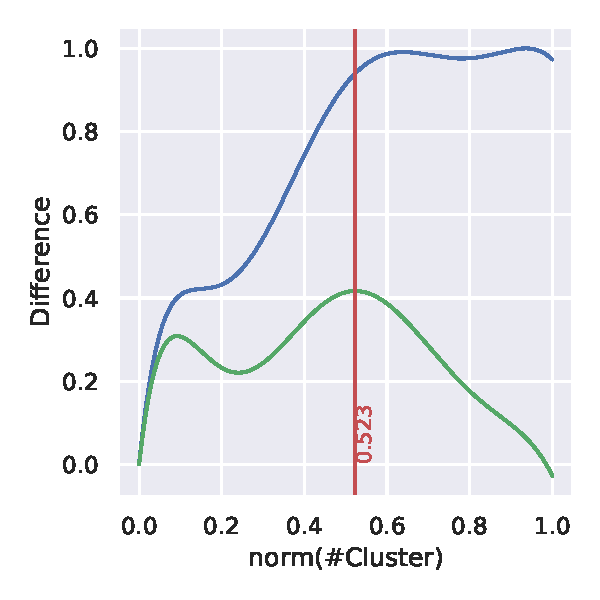
\includegraphics[width=\textwidth]{UMAP/Cluster_Knee_Segment_4.pdf}
    \end{subfigure}
    \hfill
    \begin{subfigure}[b]{0.475\textwidth}
        \caption[Kneedle Knee]{\textbf{Kneedle Knee}}
        \label{subfig:UMAP_Cluster_Knee_Elbow_4}            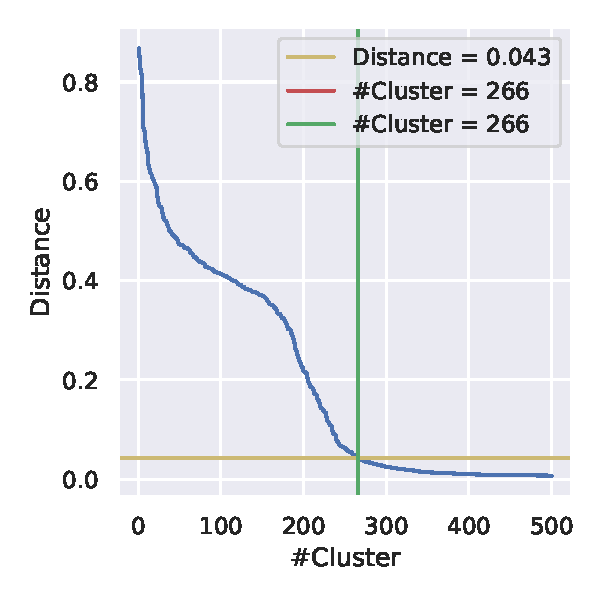
\includegraphics[width=\textwidth]{UMAP/Cluster_Elbow_Knee_Segment_4.pdf}
    \end{subfigure}
    \vskip\baselineskip
    \begin{subfigure}[b]{0.475\textwidth}
        \caption[Cluster Distribution]{\textbf{Cluster Distribution}}
        \label{subfig:UMAP_Cluster_Knee_Distributione_4}            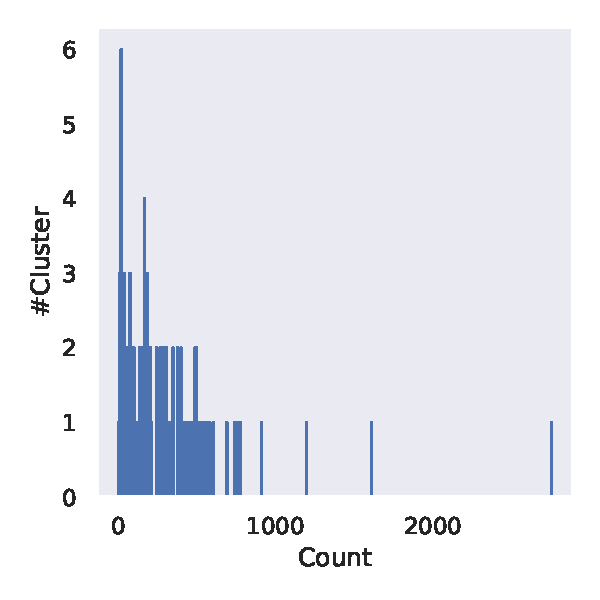
\includegraphics[width=\textwidth]{UMAP/Cluster_Distribution_Segment_4.pdf}
    \end{subfigure}
    \hfill
    \begin{subfigure}[b]{0.475\textwidth}
        \caption[Logarithmic Distribution]{\textbf{Logarithmic Distribution}}
        \label{subfig:UMAP_Cluster_Knee_Distribution_log_4}            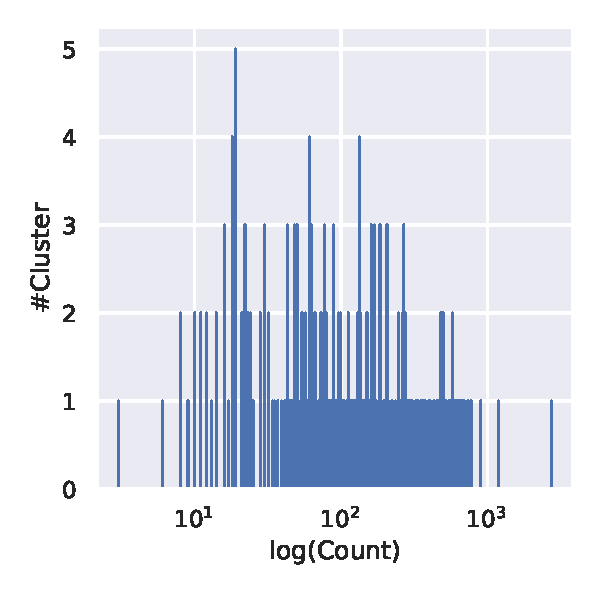
\includegraphics[width=\textwidth]{UMAP/Cluster_Distribution_Log_Segment_4.pdf}
    \end{subfigure}
    %\end{adjustbox}
    \caption[Knee based Segment 4 Clustering (\Acrshort{UMAP})]{\textbf{Knee based Segment 4 Clustering (\Acrshort{UMAP}).}.}
    \label{fig:UMAP_Cluster_Knee_4}
\end{figure}

\begin{figure}[!hbt]
    \centering
    %\begin{adjustbox}{minipage=\dimexpr\textwidth-2\fboxsep-2\fboxrule,fbox}
    \begin{subfigure}[b]{0.475\textwidth}
        \caption[Kneedle Algorithm]{\textbf{Kneedle Algorithm}}
        \label{subfig:PCA_Cluster_Knee_Kneedle_4}            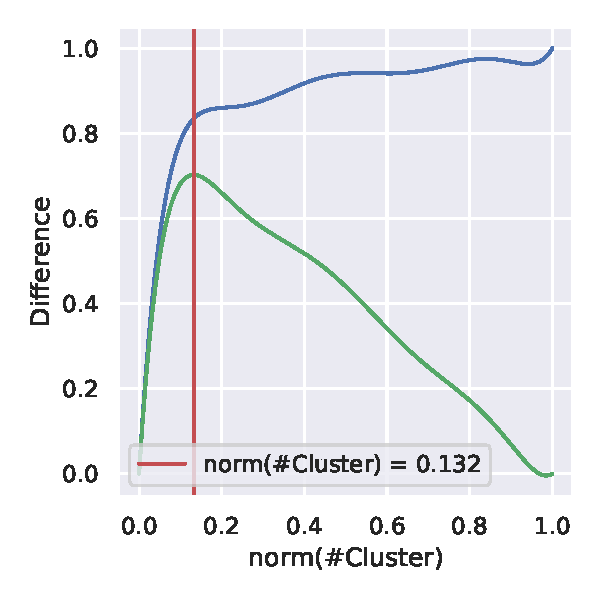
\includegraphics[width=\textwidth]{PCA/Cluster_Knee_Segment_4.pdf}
    \end{subfigure}
    \hfill
    \begin{subfigure}[b]{0.475\textwidth}
        \caption[Kneedle Knee]{\textbf{Kneedle Knee}}
        \label{subfig:PCA_Cluster_Knee_Elbow_4}            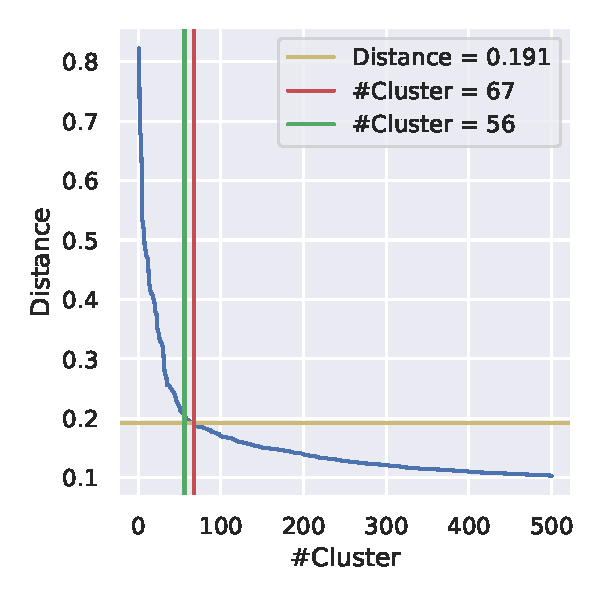
\includegraphics[width=\textwidth]{PCA/Cluster_Elbow_Knee_Segment_4.pdf}
    \end{subfigure}
    \vskip\baselineskip
    \begin{subfigure}[b]{0.475\textwidth}
        \caption[Cluster Distribution]{\textbf{Cluster Distribution}}
        \label{subfig:PCA_Cluster_Knee_Distributione_4}            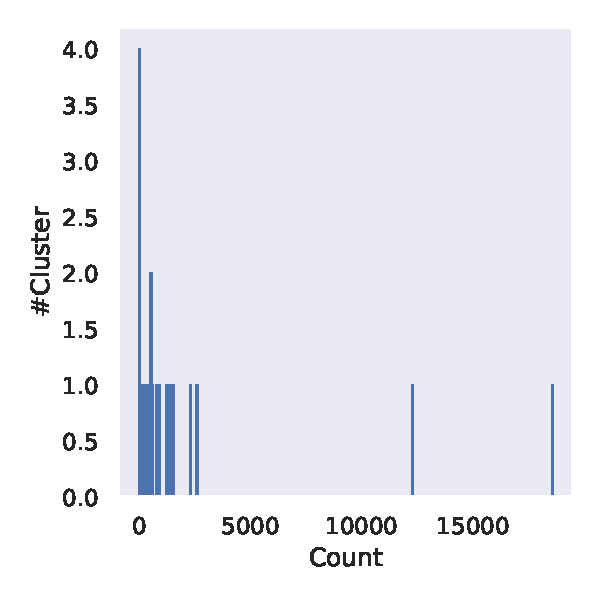
\includegraphics[width=\textwidth]{PCA/Cluster_Distribution_Segment_4.pdf}
    \end{subfigure}
    \hfill
    \begin{subfigure}[b]{0.475\textwidth}
        \caption[Logarithmic Distribution]{\textbf{Logarithmic Distribution}}
        \label{subfig:PCA_Cluster_Knee_Distribution_log_4}            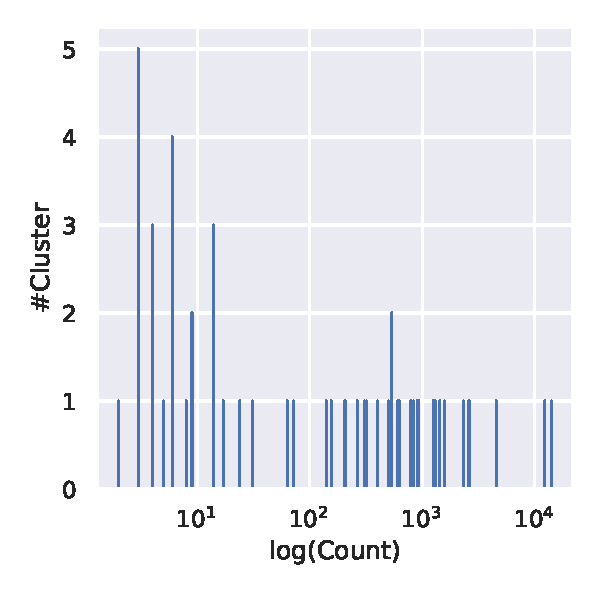
\includegraphics[width=\textwidth]{PCA/Cluster_Distribution_Log_Segment_4.pdf}
    \end{subfigure}
    %\end{adjustbox}
    \caption[Knee based Segment 4 Clustering (\Acrshort{PCA})]{\textbf{Knee based Segment 4 Clustering (\Acrshort{PCA}).}.}
    \label{fig:PCA_Cluster_Knee_4}
\end{figure}

\begin{figure}[!hbt]
    \centering
    %\begin{adjustbox}{minipage=\dimexpr\textwidth-2\fboxsep-2\fboxrule,fbox}
    \begin{subfigure}[b]{0.475\textwidth}
        \caption[\Acrshort{DBCV} Exploration]{\textbf{\Acrshort{DBCV} Exploration}}
        \label{subfig:PCA_Cluster_DBCV_Explo_4}            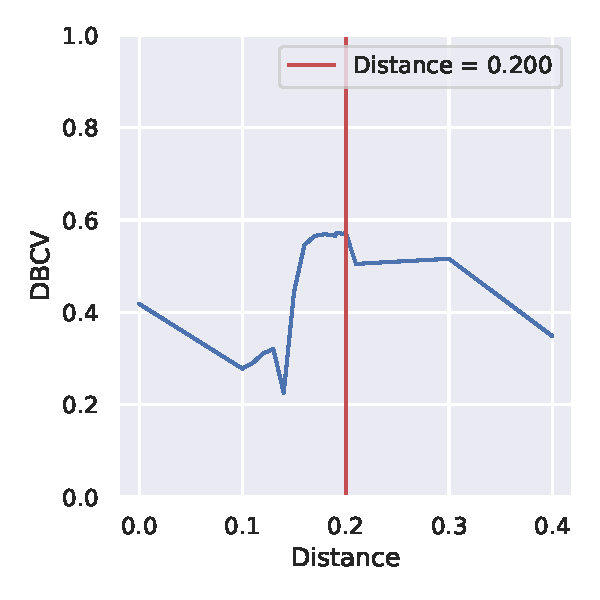
\includegraphics[width=\textwidth]{PCA/Cluster_DBCV_Segment_4.pdf}
    \end{subfigure}
    \hfill
    \begin{subfigure}[b]{0.475\textwidth}
        \caption[\Acrshort{DBCV} Knee]{\textbf{\Acrshort{DBCV} Knee}}
        \label{subfig:PCA_Cluster_DBCV_Elbow_4}            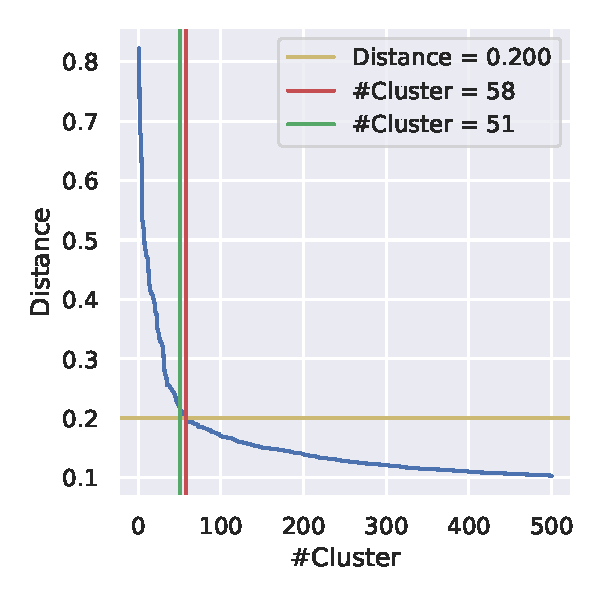
\includegraphics[width=\textwidth]{PCA/Cluster_Elbow_DBCV_Segment_4.pdf}
    \end{subfigure}
    \vskip\baselineskip
    \begin{subfigure}[b]{0.475\textwidth}
        \caption[Cluster Distribution]{\textbf{Cluster Distribution}}
        \label{subfig:PCA_Cluster_DBCV_Distribution_4}            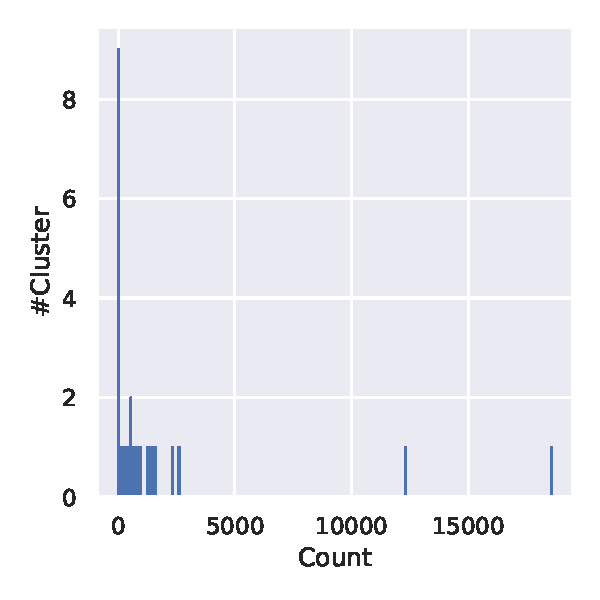
\includegraphics[width=\textwidth]{PCA/Cluster_Distribution_Segment_4_alternative.pdf}
    \end{subfigure}
    \hfill
    \begin{subfigure}[b]{0.475\textwidth}
        \caption[Logarithmic Distribution]{\textbf{Logarithmic Distribution}}
        \label{subfig:PCA_Cluster_DBCV_Distribution_log_4}            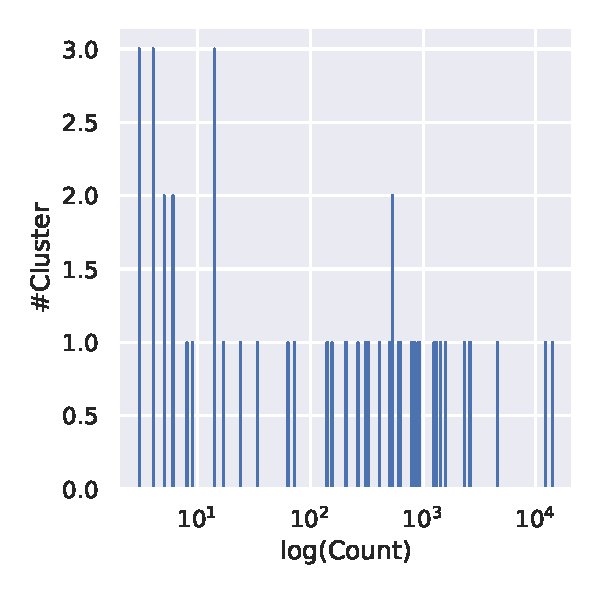
\includegraphics[width=\textwidth]{PCA/Cluster_Distribution_Log_Segment_4_alternative.pdf}
    \end{subfigure}
    %\end{adjustbox}
    \caption[\Acrshort{DBCV} based Segment 4 Clustering (\Acrshort{PCA})]{\textbf{\Acrshort{DBCV} based Segment 4 Clustering (\Acrshort{PCA}).}.}
    \label{fig:PCA_Cluster_DBCV_4}
\end{figure}

\begin{figure}[!hbt]
    \centering
    %\begin{adjustbox}{minipage=\dimexpr\textwidth-2\fboxsep-2\fboxrule,fbox}
    \begin{subfigure}[b]{0.475\textwidth}
        \caption[\Acrshort{DBCV} Exploration]{\textbf{\Acrshort{DBCV} Exploration}}
        \label{subfig:UMAP_Cluster_DBCV_Explo_4}            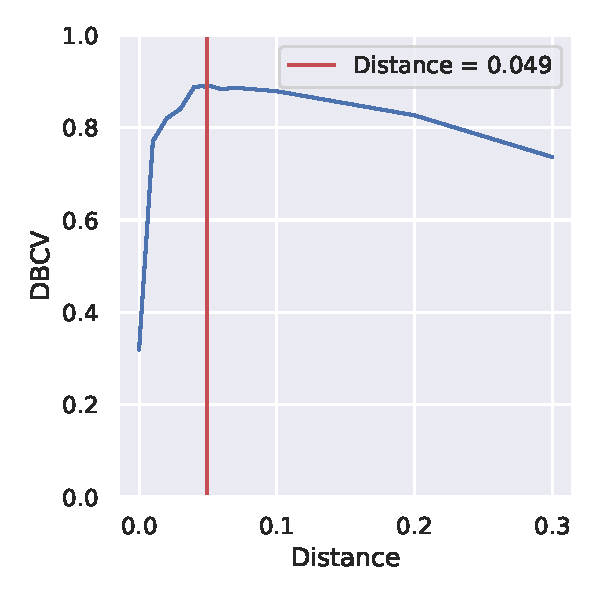
\includegraphics[width=\textwidth]{UMAP/Cluster_DBCV_Segment_4.pdf}
    \end{subfigure}
    \hfill
    \begin{subfigure}[b]{0.475\textwidth}
        \caption[\Acrshort{DBCV} Knee]{\textbf{\Acrshort{DBCV} Knee}}
        \label{subfig:UMAP_Cluster_DBCV_Elbow_4}            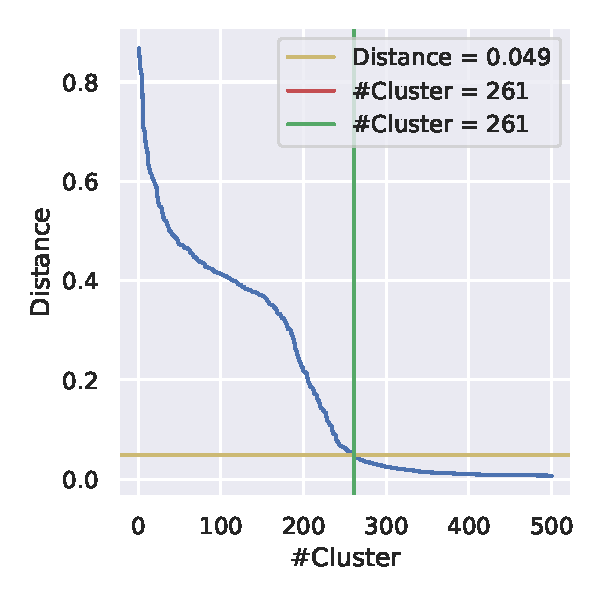
\includegraphics[width=\textwidth]{UMAP/Cluster_Elbow_DBCV_Segment_4.pdf}
    \end{subfigure}
    \vskip\baselineskip
    \begin{subfigure}[b]{0.475\textwidth}
        \caption[Cluster Distribution]{\textbf{Cluster Distribution}}
        \label{subfig:UMAP_Cluster_DBCV_Distribution_4}            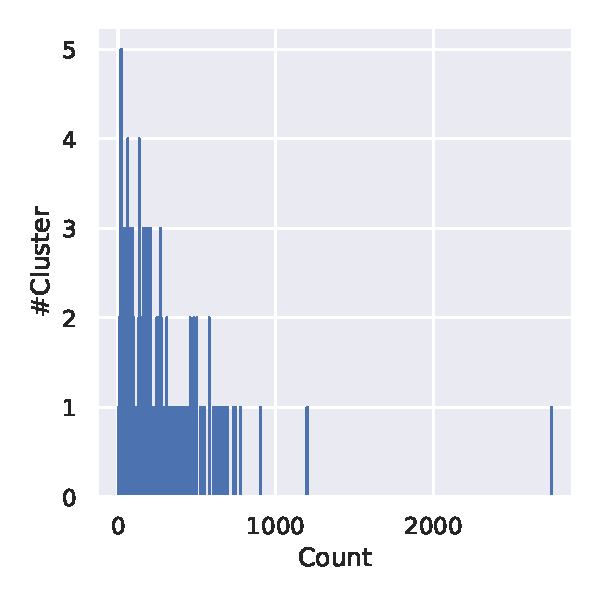
\includegraphics[width=\textwidth]{UMAP/Cluster_Distribution_Segment_4_alternative.pdf}
    \end{subfigure}
    \hfill
    \begin{subfigure}[b]{0.475\textwidth}
        \caption[Logarithmic Distribution]{\textbf{Logarithmic Distribution}}
        \label{subfig:UMAP_Cluster_DBCV_Distribution_log_4}            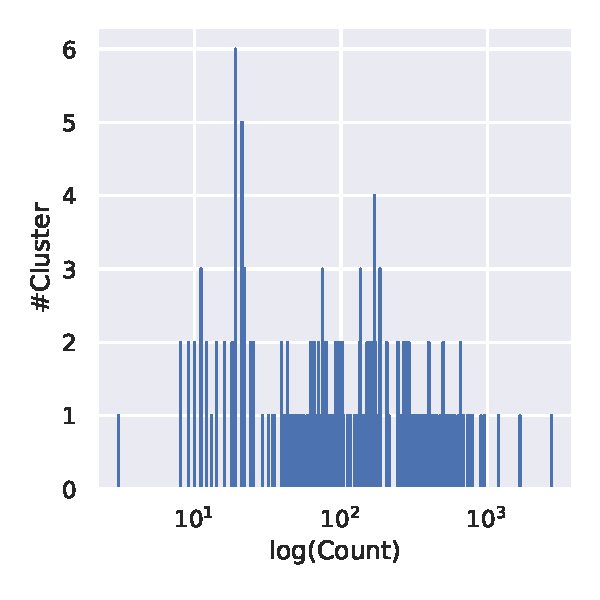
\includegraphics[width=\textwidth]{UMAP/Cluster_Distribution_Log_Segment_4_alternative.pdf}
    \end{subfigure}
    %\end{adjustbox}
    \caption[\Acrshort{DBCV} based Segment 4 Clustering (\Acrshort{UMAP})]{\textbf{\Acrshort{DBCV} based Segment 4 Clustering (\Acrshort{UMAP}).}.}
    \label{fig:UMAP_Cluster_DBCV_4}
\end{figure}




\subsection{Clustertrees}

\begin{figure}[!hbt]
    \centering
    \begin{tikzpicture}
        \node[anchor=south west,inner sep=0] (image) at (0,0) {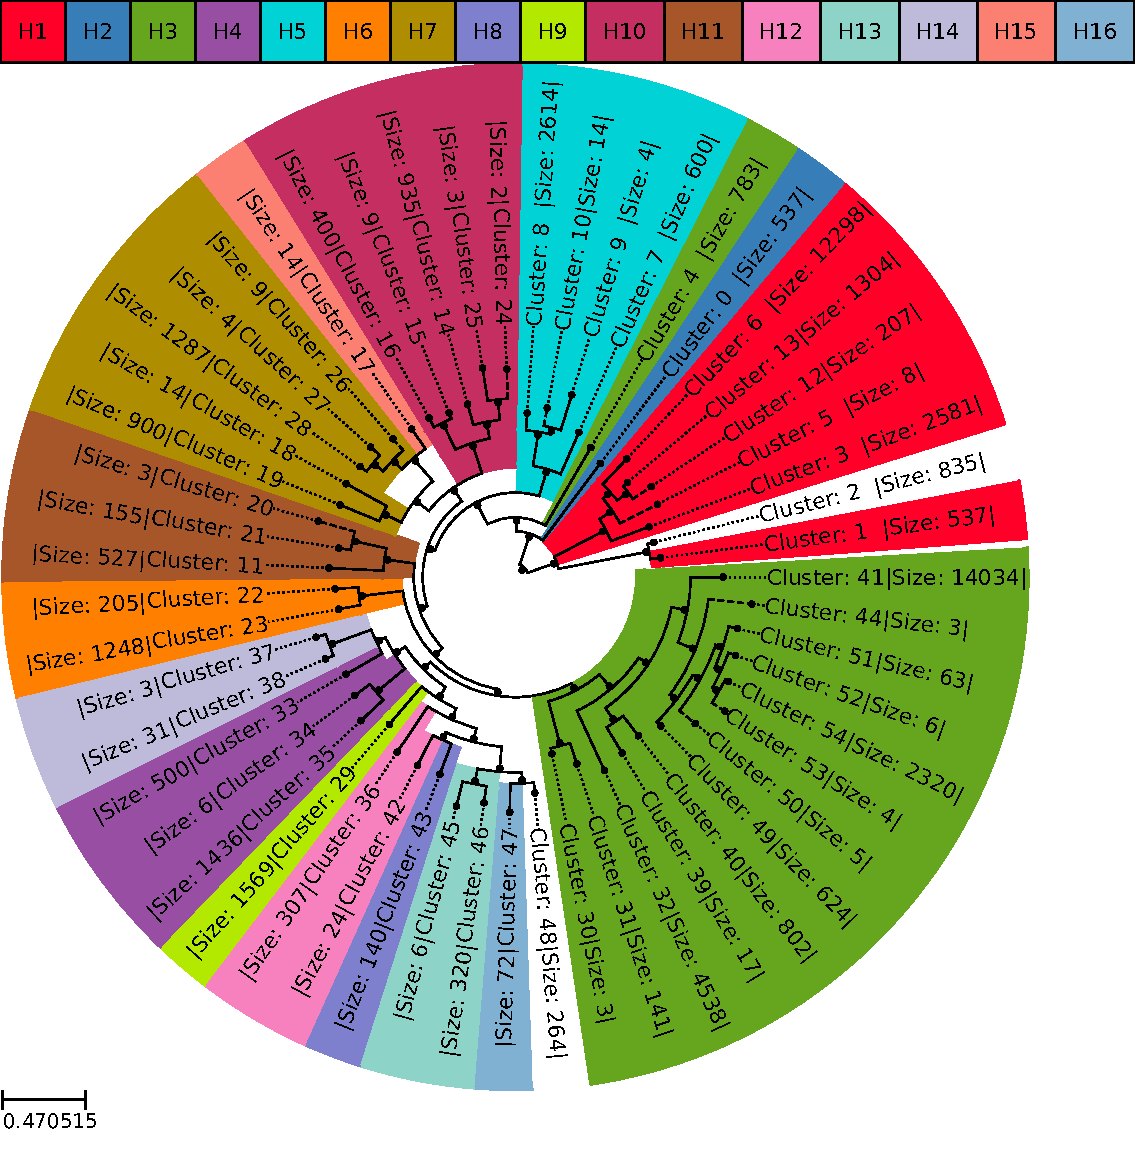
\includegraphics[width=\textwidth]{PCA/Clustertree_Segment_4_H_Knee.pdf}};
        \begin{scope}[x={(image.south east)},y={(image.north west)}]
            %\draw[help lines,xstep=.1,ystep=.1] (0,0) grid (1,1);
            %\draw[black, thick,rounded corners] (7.5,5.3) rectangle (9.4,6.2);
        \end{scope}
    \end{tikzpicture}

    \caption[Knee based Segment 4 Clustertree (\Acrshort{PCA})]{\textbf{Knee based Segment 4 Clustertree (\Acrshort{PCA}).} .}
    \label{fig:PCA_Clusteree_Knee_4}
\end{figure}

\begin{figure}[!hbt]
    \centering
    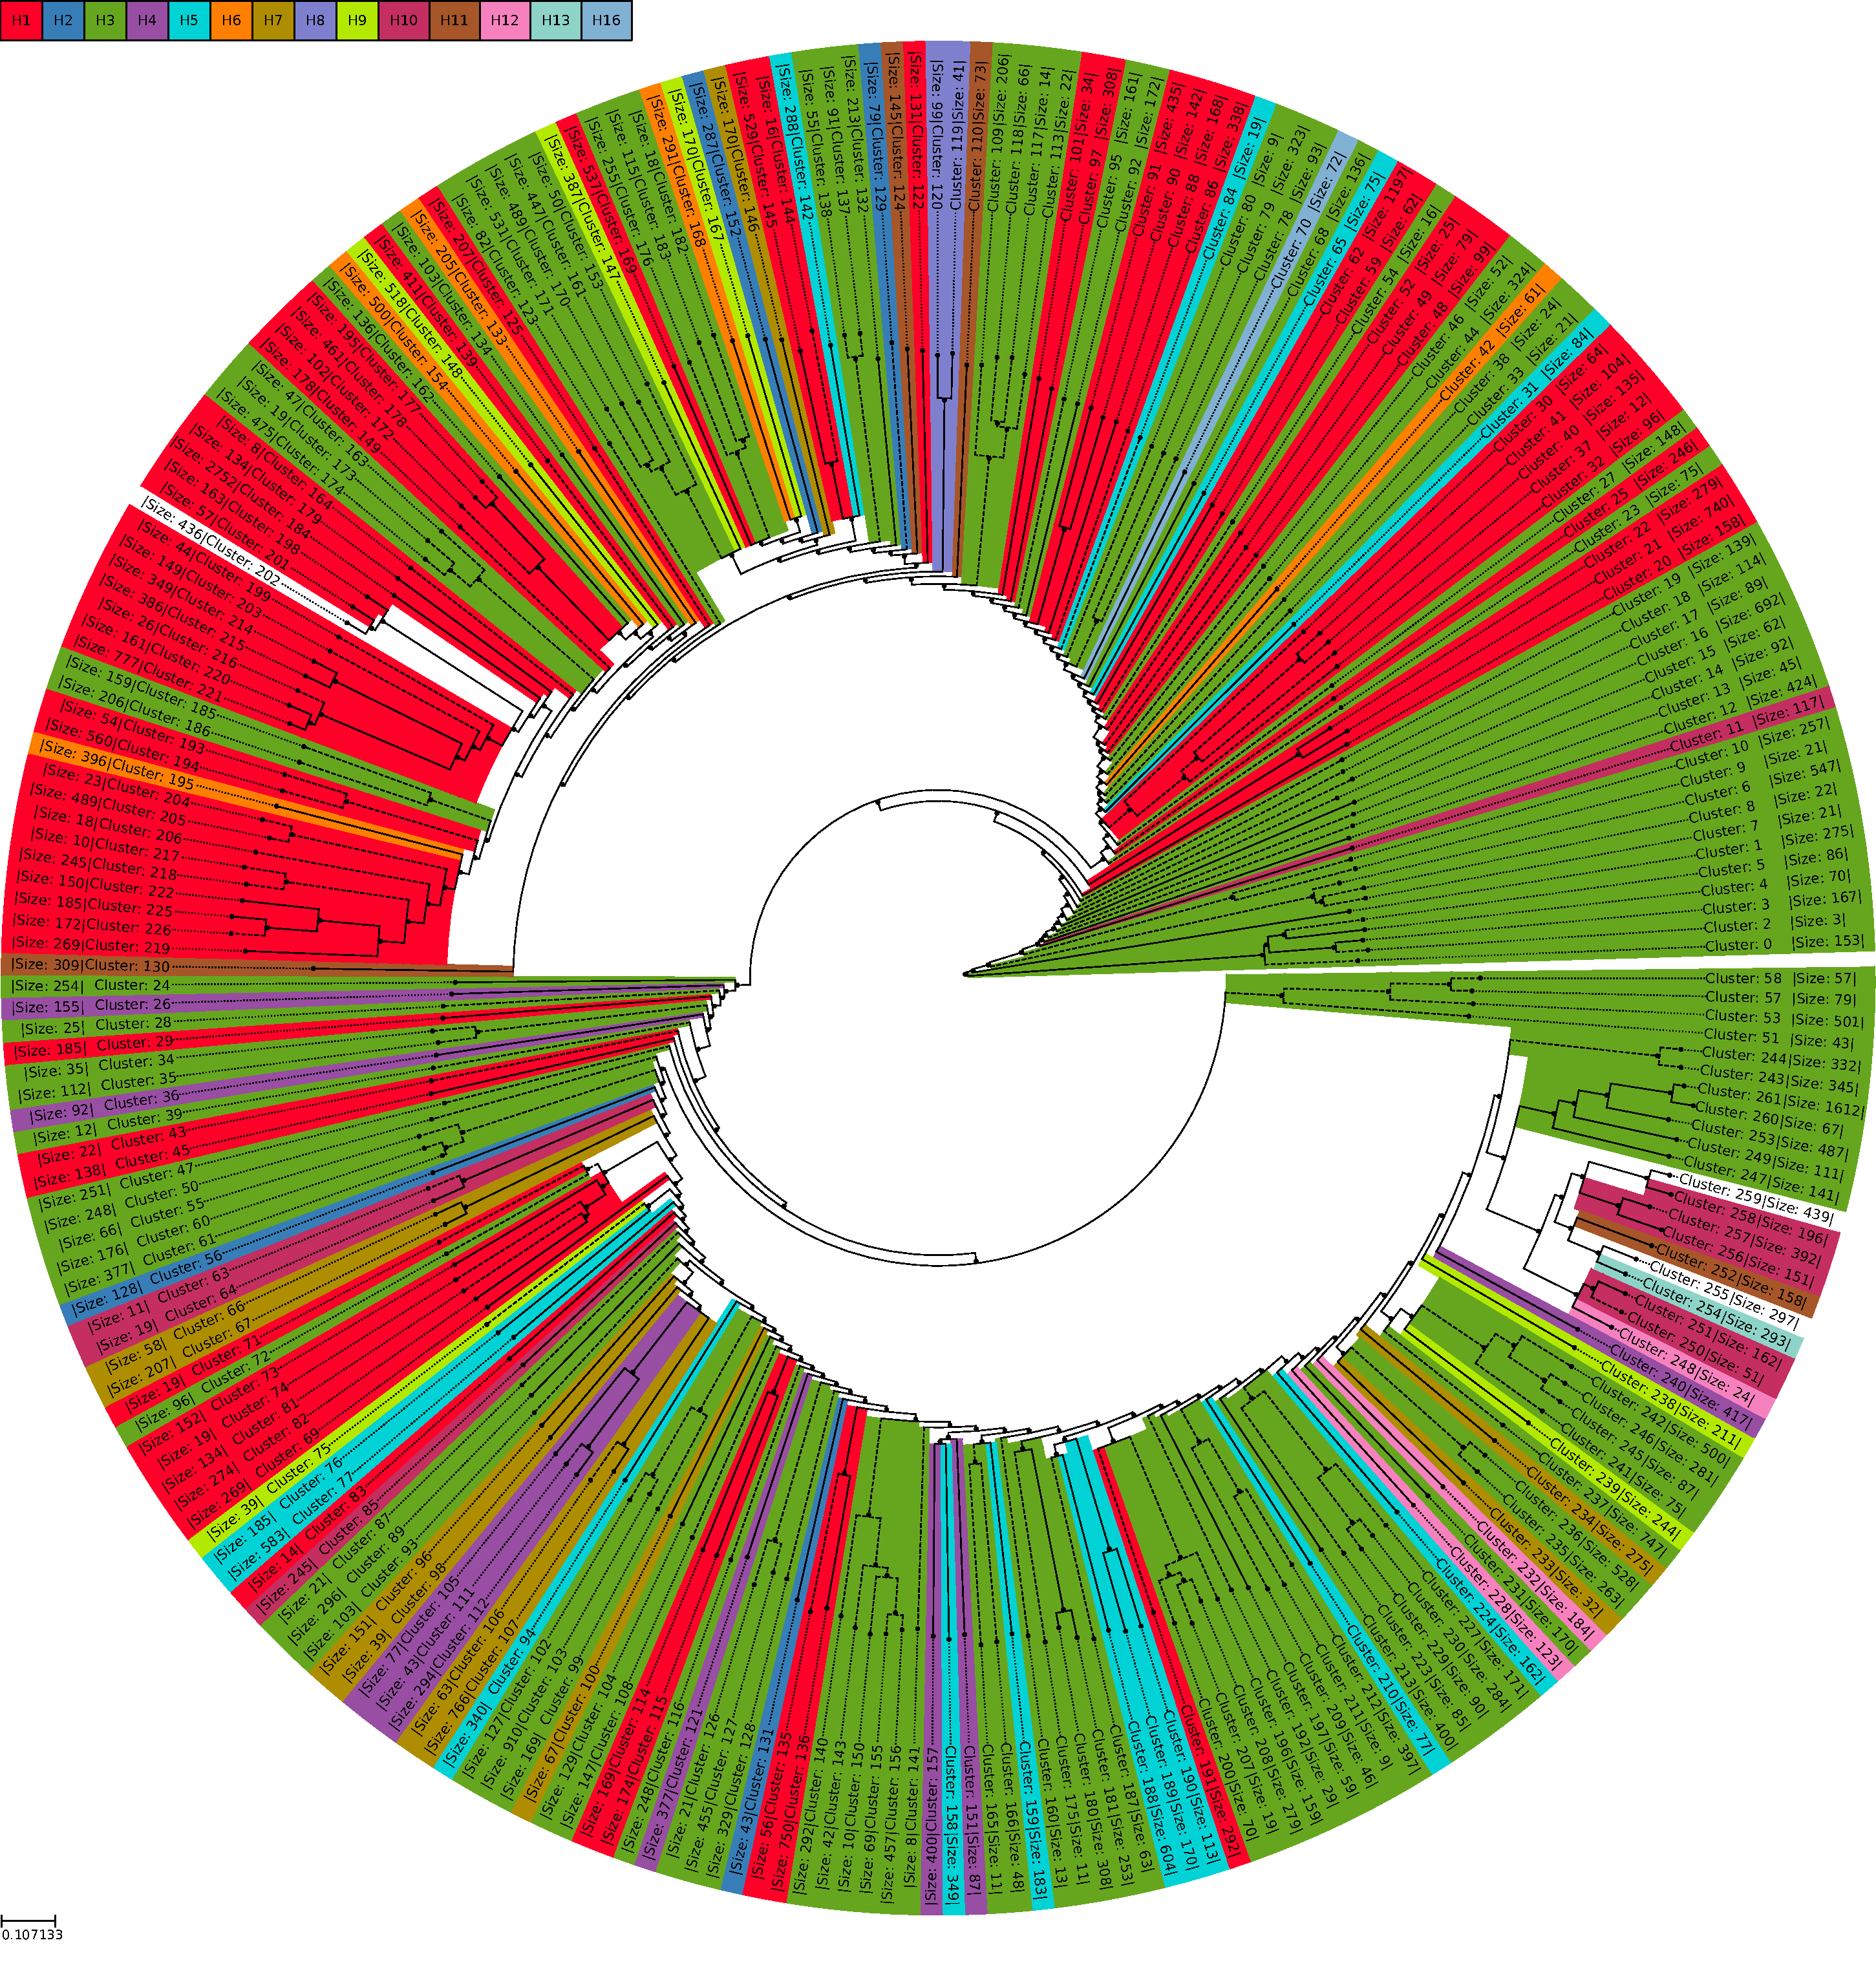
\includegraphics[width=\textwidth]{UMAP/Clustertree_Segment_4_H_Knee.pdf}
    \caption[Knee based Segment 4 Clustertree (\Acrshort{UMAP})]{\textbf{Knee based Segment 4 Clustertree (\Acrshort{UMAP}).} .}
    \label{fig:UMAP_Clusteree_Knee_4}
\end{figure}